\documentclass[10pt]{exam}

\usepackage{amsmath, amssymb, multicol}
\usepackage{graphicx}
\usepackage{textcomp}
\usepackage{chessboard}
\usepackage{tikz}

\def\d{\displaystyle}
\def\b{\mathbf}
\def\R{\mathbf{R}}
\def\Z{\mathbf{Z}}
\def\st{~:~}
\def\bar{\overline}
\def\inv{^{-1}}
\def\r{2.5pt}
\def\v{circle (\r)}


%\pointname{pts}
\pointsinmargin
\marginpointname{pts}
\addpoints
\pagestyle{head}
\printanswers

\firstpageheader{Math 228}{\bf Graph Sameness}{Friday, November 3}


\begin{document}

%space for name
%\noindent {\large\bf Name:} \underline{\hspace{2.5in}}
%\vskip 1em
\noindent{\bf Main Question}: What does it mean for two graphs to be the same?

\begin{questions}
\question Which (if any) of the graphs below are the same?


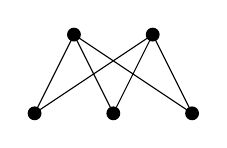
\begin{tikzpicture}
\coordinate (A) at (-1,0);
\coordinate (B) at (0,0);
\coordinate (C) at (1,0);
\coordinate (D) at (-.5,1);
\coordinate (E) at (.5,1);

\draw (A) -- (D) -- (B) -- (E) -- (C) -- (D)  (A) -- (E);
\foreach \x in {(A), (B), (C), (D), (E)}{
	\fill \x \v;
}
\end{tikzpicture}
\hfill
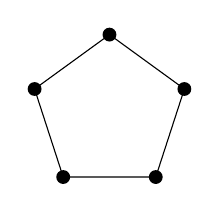
\begin{tikzpicture}
\coordinate (A) at (90+360/5:1);
\coordinate (B) at (90+2*360/5:1);
\coordinate (C) at (90+3*360/5:1);
\coordinate (D) at (90+4*360/5:1);
\coordinate (E) at (90:1);

\draw (A) -- (B) -- (C) -- (D) -- (E) -- (A);
\foreach \x in {(A), (B), (C), (D), (E)}{
	\fill \x \v;
}
\end{tikzpicture}
\hfill
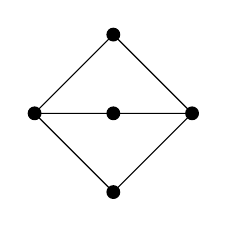
\begin{tikzpicture}
\coordinate (A) at (-1,0);
\coordinate (B) at (0,1);
\coordinate (C) at (0,0);
\coordinate (D) at (0,-1);
\coordinate (E) at (1,0);

\draw (A) -- (B) -- (E) -- (C) -- (A) -- (D) -- (E);
\foreach \x in {(A), (B), (C), (D), (E)}{
	\fill \x \v;
}
\end{tikzpicture}
\hfill
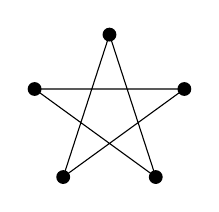
\begin{tikzpicture}
\coordinate (A) at (90+360/5:1);
\coordinate (B) at (90+2*360/5:1);
\coordinate (C) at (90+3*360/5:1);
\coordinate (D) at (90+4*360/5:1);
\coordinate (E) at (90:1);

\draw (A) -- (C) -- (E) -- (B) -- (D) -- (A);
\foreach \x in {(A), (B), (C), (D), (E)}{
	\fill \x \v;
}
\end{tikzpicture}
\hfill
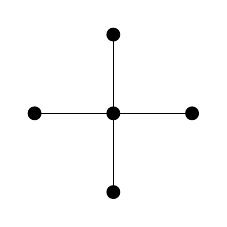
\begin{tikzpicture}
\coordinate (A) at (-1,0);
\coordinate (B) at (0,1);
\coordinate (C) at (0,0);
\coordinate (D) at (0,-1);
\coordinate (E) at (1,0);

\draw (A) -- (C) -- (B) (D) -- (C) -- (E);
\foreach \x in {(A), (B), (C), (D), (E)}{
	\fill \x \v;
}
\end{tikzpicture}
\hfill
~

\begin{solution}
The first and third graphs are different drawings of the same graph.  The second and fourth are also just different ways to draw the same graph.  The fifth graph is not the same as any other (for example, we see that it has a vertex of degree 4, but none of the other graphs have this property).
\end{solution}
\vfill

\question The graphs above are unlabeled.  Usually we think of a graph as having a specific set of vertices.  Which (if any) of the graphs below are the same?

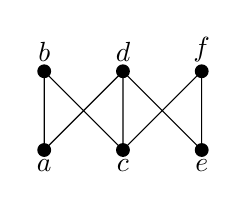
\begin{tikzpicture}
\coordinate (A) at (-1,0);
\coordinate (B) at (-1, 1);
\coordinate (C) at (0,0);
\coordinate (D) at (0,1);
\coordinate (E) at (1,0);
\coordinate (F) at (1,1);

\draw (A) node[below] {$a$} -- (B) node[above] {$b$} -- (C) node[below] {$c$} -- (D) node[above] {$d$} -- (E) node[below] {$e$} -- (F) node[above] {$f$} -- (C) (A) -- (D);
\foreach \x in {(A), (B), (C), (D), (E), (F)}{
	\fill \x \v;
}
\end{tikzpicture}
\hfill
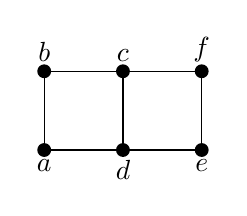
\begin{tikzpicture}
\coordinate (A) at (-1,0);
\coordinate (B) at (-1, 1);
\coordinate (C) at (0,1);
\coordinate (D) at (0,0);
\coordinate (E) at (1,0);
\coordinate (F) at (1,1);

\draw (A) node[below] {$a$} -- (B) node[above] {$b$} -- (C) node[above] {$c$} -- (D) node[below] {$d$} -- (E) node[below] {$e$} -- (F) node[above] {$f$} -- (C) (A) -- (D);
\foreach \x in {(A), (B), (C), (D), (E), (F)}{
	\fill \x \v;
}
\end{tikzpicture}
\hfill
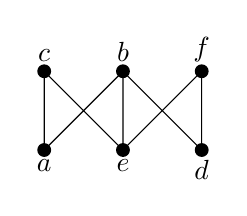
\begin{tikzpicture}
\coordinate (A) at (-1,0);
\coordinate (B) at (-1, 1);
\coordinate (C) at (0,0);
\coordinate (D) at (0,1);
\coordinate (E) at (1,0);
\coordinate (F) at (1,1);

\draw (A) node[below] {$a$} -- (B) node[above] {$c$} -- (C) node[below] {$e$} -- (D) node[above] {$b$} -- (E) node[below] {$d$} -- (F) node[above] {$f$} -- (C) (A) -- (D);
\foreach \x in {(A), (B), (C), (D), (E), (F)}{
	\fill \x \v;
}
\end{tikzpicture}
\hfill
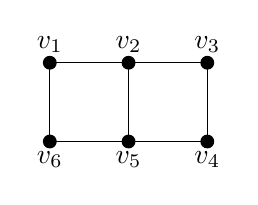
\begin{tikzpicture}
\coordinate (A) at (-1,0);
\coordinate (B) at (-1, 1);
\coordinate (C) at (0,1);
\coordinate (D) at (0,0);
\coordinate (E) at (1,0);
\coordinate (F) at (1,1);

\draw (A) node[below] {$v_6$} -- (B) node[above] {$v_1$} -- (C) node[above] {$v_2$} -- (D) node[below] {$v_5$} -- (E) node[below] {$v_4$} -- (F) node[above] {$v_3$} -- (C) (A) -- (D);
\foreach \x in {(A), (B), (C), (D), (E), (F)}{
	\fill \x \v;
}
\end{tikzpicture}

\begin{solution}
If you drag the vertices $d$ and $c$ of the first graph so that they swap places, you get exactly the second graph.  These two graphs are equal.  The other two graphs look the same, but their labels are different.  We say that these last two are \emph{isomorphic} to each other (and to the first two graphs) because there is a way to relabel the vertices to get the other graphs.  In other words, we must give a function from the vertices of one to the vertices of the other.  But the key thing is that vertices that are \emph{adjacent} in the first graph must correspond to vertices that are adjacent in the second graph.

For example, go from the second graph to the fourth by $f(b) = v_1$, $f(a) = v_6$, $f(c) = v_2$, $v(d) = v_5$, $f(f) = v_3$, $f(e) = v_4$.

\end{solution}

\vfill

\question Actually, all the graphs we have seen above are just {\em drawings} of graphs.  A graph is really an abstract mathematical object consisting of two sets $V$ and $E$ where $E$ is a set of 2-element subsets of $V$.
\vskip 1ex
Are the graphs below the same or different?
\vskip 1em
Graph 1: $V = \{a, b, c, d, e\}$, $E = \{\{a,b\}, \{a, c\}, \{a,d\}, \{a,e\}, \{b,c\}, \{d,e\}\}$.
\vskip 1ex

Graph 2: $V = \{v_1, v_2, v_3, v_4, v_5\}$, $E = \{\{v_1, v_3\}, \{v_1, v_5\}, \{v_2, v_4\}, \{v_2, v_5\}, \{v_3, v_5\}, \{v_4, v_5\}\}$.

\begin{solution}
The graph are not equal (they have different sets for $V$) but they \emph{are} isomorphic.  This is fairly easy to see if you draw both graphs, and that suggests how to create the isomorphism (the relabeling function).

We must send $a$ to a vertex that is adjacent to every other vertex: so pick $v_5$.  We can then send $b$ to $v_1$.  In the first graph, $b$ is also adjacent to $c$, so we should send $c$ to something adjacent to $v_1$, thus send $c$ to $v_3$.  Finally we can send $d$ to $v_2$ and $e$ to $v_4$.
\end{solution}
\vfill


\newpage

\uplevel{For each of the following, try to give two \underline{different} unlabeled graphs with the given properties, or explain why doing so is impossible.}

\question Two different trees with the same number of vertices and the same number of edges.
\begin{solution} For example, the following trees both have 5 vertices and 4 edges, but one has a vertex of degree 4 and the other does not:

\begin{center}
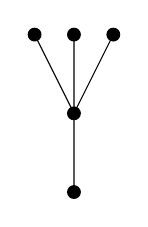
\begin{tikzpicture}
\coordinate (A) at (0,0);
\coordinate (B) at (0,1);
\coordinate (C) at (-.5,2);
\coordinate (D) at (0,2);
\coordinate (E) at (.5,2);

\draw (A) -- (B) -- (C) (B) -- (D) (B) -- (E);
\foreach \x in {(A), (B), (C), (D), (E)}{
	\fill \x \v;
}
\end{tikzpicture}
\hspace{.3\textwidth}
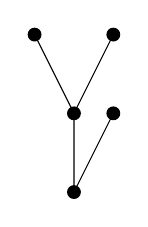
\begin{tikzpicture}
\coordinate (A) at (0,0);
\coordinate (B) at (0,1);
\coordinate (C) at (-.5,2);
\coordinate (D) at (.5,1);
\coordinate (E) at (.5,2);

\draw (A) -- (B) -- (C) (A) -- (D) (B) -- (E);
\foreach \x in {(A), (B), (C), (D), (E)}{
	\fill \x \v;
}
\end{tikzpicture}
\end{center}
\end{solution}
\vfill
\question Two different graphs with 8 vertices all of degree 2.

\begin{solution} Note that graphs do not need to be \emph{connected}.  The graph on the right below looks like two squares, but together they can be considered one graph.

\begin{center}
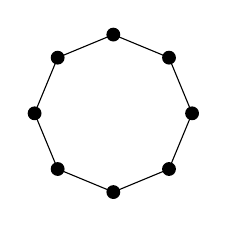
\begin{tikzpicture}
\foreach \x in {0,...,7}{
	\coordinate (A\x) at (\x*360/8:1);
	\coordinate (B\x) at (\x*360/8+360/8:1);
	\draw (A\x) -- (B\x);
	\fill (A\x) \v;
}


\end{tikzpicture}
\hspace{.3\textwidth}
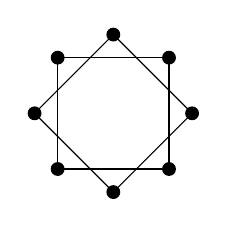
\begin{tikzpicture}
\foreach \x in {0,...,7}{
	\coordinate (A\x) at (\x*360/8:1);
	\coordinate (B\x) at (\x*360/8+2*360/8:1);
	\draw (A\x) -- (B\x);
	\fill (A\x) \v;
}


\end{tikzpicture}
\end{center}
\end{solution}
\vfill
\question Two different graphs with 5 vertices all of degree 4.
\begin{solution}
This is not possible.  If the graph has 5 vertices, and all vertices have degree 4, then each vertex is adjacent to every other vertex.  This means the graph is $K_5$.
\end{solution}
\vfill
\question Two different graphs with 5 vertices all of degree 3.
\begin{solution}
This is also not possible, but for a different reason: there are no graphs at all that have this property.  The reason is that such a group would have 15/2 edges, which is not a whole number.
\end{solution}
\vfill
\uplevel{When a connected graph can be drawn without any edges crossing, it is called {\em planar}.  When a planar graph is drawn in this way, it divides the plane into regions called {\em faces}.}
\question Two different planar graphs with the same number of vertices, edges, and faces.

\begin{solution} For example:

\begin{center}
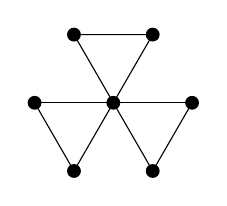
\begin{tikzpicture}
\coordinate (A) at (0,0);
\coordinate (B) at (60:1);
\coordinate (C) at (120:1);
\coordinate (D) at (180:1);
\coordinate (E) at (240:1);
\coordinate (F) at (300:1);
\coordinate (G) at (0:1);

\draw (B) -- (C) (D) -- (E) (F) -- (G);
\foreach \x in {(B), (C), (D), (E), (F), (G)}{
\draw (A) -- \x;
	\fill \x \v;
}
\fill (A) \v;
\end{tikzpicture}
\hspace{.3\textwidth}
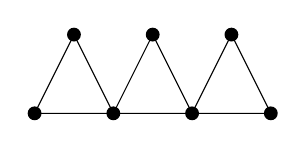
\begin{tikzpicture}
\coordinate (A) at (0,0);
\coordinate (B) at (1,0);
\coordinate (C) at (2,0);
\coordinate (D) at (3,0);
\coordinate (E) at (.5,1);
\coordinate (F) at (1.5,1);
\coordinate (G) at (2.5,1);

\draw (A) -- (B) -- (C) -- (D) -- (G) -- (C)  -- (F) -- (B) -- (E) -- (A);
\foreach \x in {(A), (B), (C), (D), (E), (F), (G)}{
	\fill \x \v;
}
\end{tikzpicture}
\end{center}
\end{solution}
\vfill

\question Two different planar graphs with the same number of vertices and edges, but a different number of faces.
\begin{solution}
This is impossible, as we will soon see using Euler's Formula.
\end{solution}


\end{questions}

% \newpage
%
% \centerline{\bf Graph Definitions}
% \begin{itemize}
%     \item[] {\bf Graph}: A collection of {\em vertices}, some of which are connected by {\em edges}.  More precisely, a pair of sets $V$ and $E$ where $V$ is a set of vertices and $E$ is a set of 2-element subsets of $V$.
%     \item[] {\bf Adjacent}: Two vertices are {\em adjacent} if they are connected by an edge.  Two edges are {\em adjacent} if they share a vertex.
%     \item[] {\bf Bipartite graph}: A graph for which it is possible to divide the vertices into two disjoint sets such that there are no edges between any two vertices in the same set.
%     \item[] {\bf Complete bipartite graph}: A bipartite graph for which every vertex in the first set is adjacent to every vertex in the second set.
%     \item[] {\bf Complete graph}: A graph in which every pair of vertices is adjacent.
%     \item[] {\bf Connected}: A graph is {\em connected} if there is a path from any vertex to any other vertex.
%     \item[] {\bf Chromatic number}: The minimum number of colors required in a proper vertex coloring of the graph.
%     \item[] {\bf Cycle}: A path (see below) that starts and stops at the same vertex, but contains no other repeated vertices.
%     \item[] {\bf Degree of a vertex}: The number of edges incident to a vertex.
%     \item[] {\bf Euler path}: A walk which uses each edge exactly once.
%     \item[] {\bf Euler circuit}: An Euler path which starts and stops at the same vertex.
%     \item[] {\bf Face}: A region in the plane bordered by edges and vertices when a planar graph is drawn without edges crossing.
% 		\item[] {\bf Incident}: A vertex and an edge are \emph{incident} when the edge ends in the vertex.  That is, if $\{x,y\}$ is an edge, $x$ and $y$ are its incident vertices.
%     \item[] {\bf Multigraph}: A {\em multigraph} is just like a graph but can contain multiple edges between two vertices as well as single edge loops (that is an edge from a vertex to itself).
%     \item[] {\bf Neighbor}: The neighbors of a vertex are all the vertices adjacent to it.
%     \item[] {\bf Path}: A sequence of vertices such that consecutive vertices (in the sequence) are adjacent (in the graph).  A path in which no vertex is repeated is called {\em simple}.
%     \item[] {\bf Planar}: A graph whcih can be drawn (in the plane) without any edges crossing.
%     \item[] {\bf Subgraph}: We say that $H$ is a subgraph of $G$ if every vertex and edge of $H$ is also a vertex or edge of $G$.  We say $H$ is an {\em induced} subgraph of $G$ if every vertex of $H$ is a vertex of $G$ and for pair of vertices in $H$ are adjacent in $H$ if and only if they are adjacent in $G$.
%     \item[] {\bf Tree}: A (connected) graph with no cycles.  (A non-connected graph with no cycles is called a {\em forest}.)  The vertices in a tree with degree 1 are called {\em leaves}.
%     \item[] {\bf Vertex coloring}: An assignment of colors to each of the vertices of a graph. A vertex coloring is {\em proper} if adjacent vertices are always colored differently.
% 		\item[] {\bf Walk}: A sequence of vertices such that consecutive vertices (in the sequence) are adjacent (in the graph).  A walk in which no vertex is repeated is called {\em simple}
%
%
%   \end{itemize}
%
%
% %
% %\vfill
% %  Some graphs are used more than others, and get special names.
% %  \begin{itemize}
% %    \item $K_n$: the complete graph on $n$ vertices.
% %    \item $K_{m,n}$: the complete bipartite graph with sets of $m$ and $n$ vertices.
% %    \item $C_n$: the cycle graph on $n$ vertices - just one big loop.
% %    \item $P_n$: the path graph on $n$ vertices - just one long path.
% %  \end{itemize}
% % % Here are some typical examples:
% %
% %\def\sb{.6}
% %\begin{center}
% %\hfill
% %\begin{tikzpicture}[scale=\sb+.05]
% %  \path (0,.9) +(18:1) coordinate (a);
% %  \path (0,.9) +(90:1) coordinate (b);
% %  \path (0,.9) +(162:1) coordinate (c);
% %  \path (0,.9) +(234:1) coordinate (d);
% %  \path (0,.9) +(306:1) coordinate (e);
% %  \draw[thick,fill=black] (a) \v -- (b) \v -- (c) \v -- (d) \v -- (e) \v;
% %  \draw[thick] (e) -- (a) -- (c) -- (e) -- (b) -- (d) -- (a);
% %  \draw (0,-.5) node[below]{\large $K_5$};
% %\end{tikzpicture}
% %\hfill
% %\begin{tikzpicture}[scale=\sb, xscale=1.5]
% % \draw[thick, fill=black] (-1, 0) \v -- (-.5,2) \v -- (0,0) \v -- (.5, 2) \v -- (1,0) \v -- (-.5,2) (.5,2) -- (-1,0);
% % \draw (0,-.5) node[below]{\large $K_{2,3}$};
% %  \end{tikzpicture}
% %\hfill
% %\begin{tikzpicture}[scale=\sb]
% %  \draw[thick, fill=black] (0:1) \v -- (60:1) \v -- (120:1) \v -- (180:1) \v -- (240:1) \v -- (300:1) \v -- (0:1);
% %  \draw (270:1.5) node[below]{\large $C_6$};
% %\end{tikzpicture}
% %\hfill
% %\begin{tikzpicture}[scale=\sb]
% %  \draw[thick, fill=black] (-2,0) \v -- (-1,.5) \v -- (0,0) \v -- (1,.75) \v -- (.5,1.5) \v -- (2,2) \v;
% %  \draw (0,-.5) node[below]{\large $P_6$};
% %\end{tikzpicture}
% %\hfill
% %~
% %\end{center}


\end{document}
